\subsection{$d(K^-, p)"\pi^-\Lambda"$ and $d(K^-, p)"\pi^-\Sigma^0"$ identification} \label{sec:KPpimpim}
\begin{figure}[htbp]
  \centering
  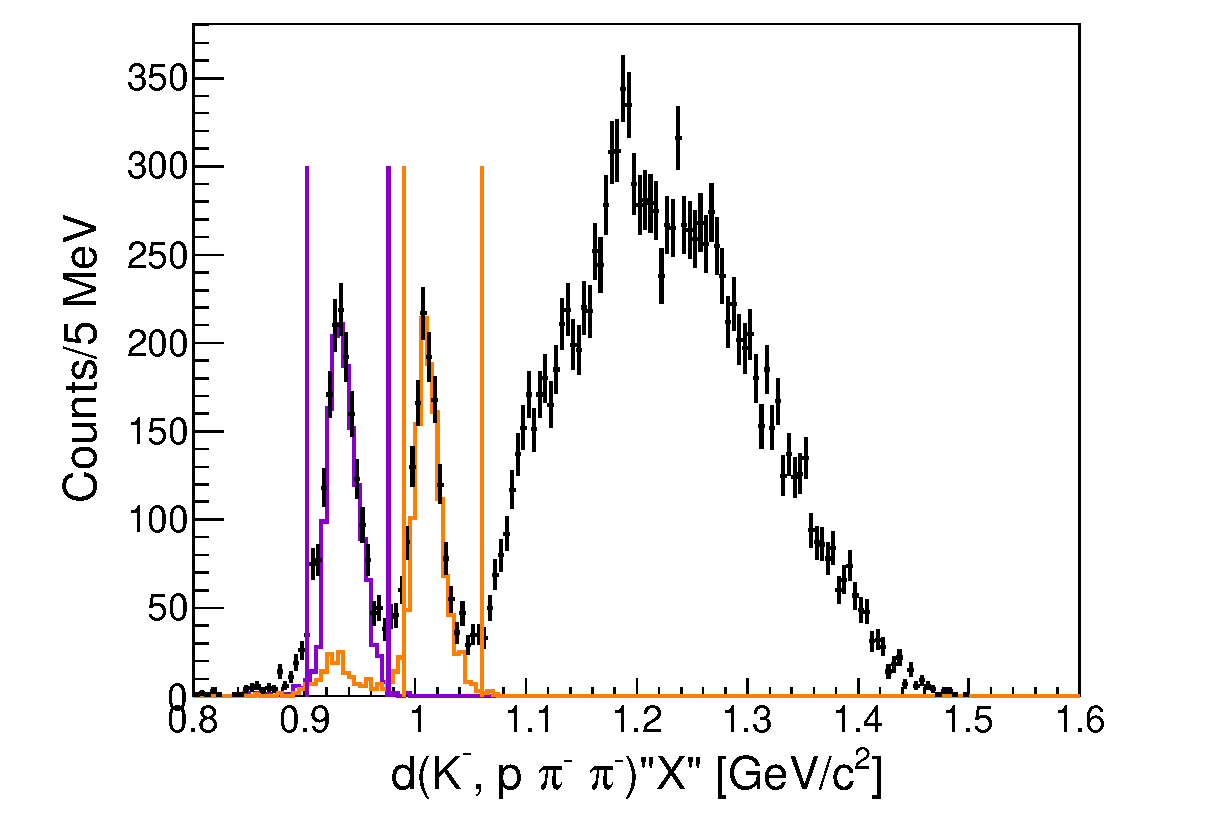
\includegraphics[width=8cm]{../pic/Run68/KP_ana/KPpimpim_MM.eps}
  \caption{
    This figure shows the missing mass of $d(K^-, p \pi^- \pi^-)$.
    Orange and purple lines indicate selection region as missing $p$ and $p \pi^-$, respectively.
    $d(K^-, p \pi^-)"\Sigma^0"$ and $d(K^-, p \pi^-)"\Lambda"$ tagged events are drawn orange and purple plot in same figure.
  }
  \label{fig:KPpimpim}
\end{figure}

\begin{figure}[htbp]
  \centering
  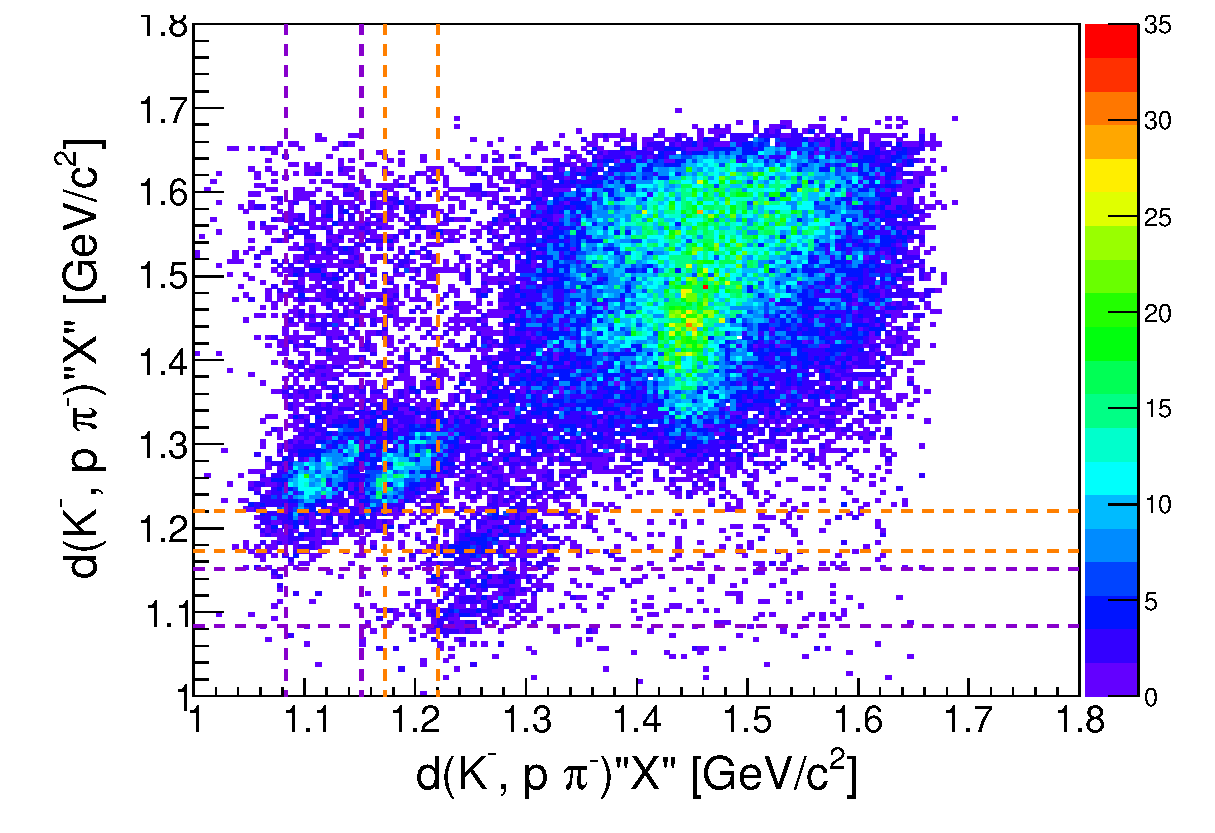
\includegraphics[width=8cm]{../pic/Run68/KP_ana/KPpim_KPpim_MM.eps}
  \caption{
    This figure shows the scatter plot of the $d(K^-, p \pi^-)$ missing masses in the $p$ and two $\pi^-$ detected events.
    Horizontal axis represents nearer DCA $\pi^-$ and virtical axis represents other one.
    Orange and purple lines indicate selection region as $d(K^-, p \pi^-)"\Sigma^0"$ and $d(K^-, p \pi^-)"\Lambda"$, respectively.
  }
  \label{fig:KPpim_KPpim}
\end{figure}

\begin{figure}[htbp]
  \centering
  \begin{tabular}{cc}
    \begin{minipage}{0.5\hsize}
      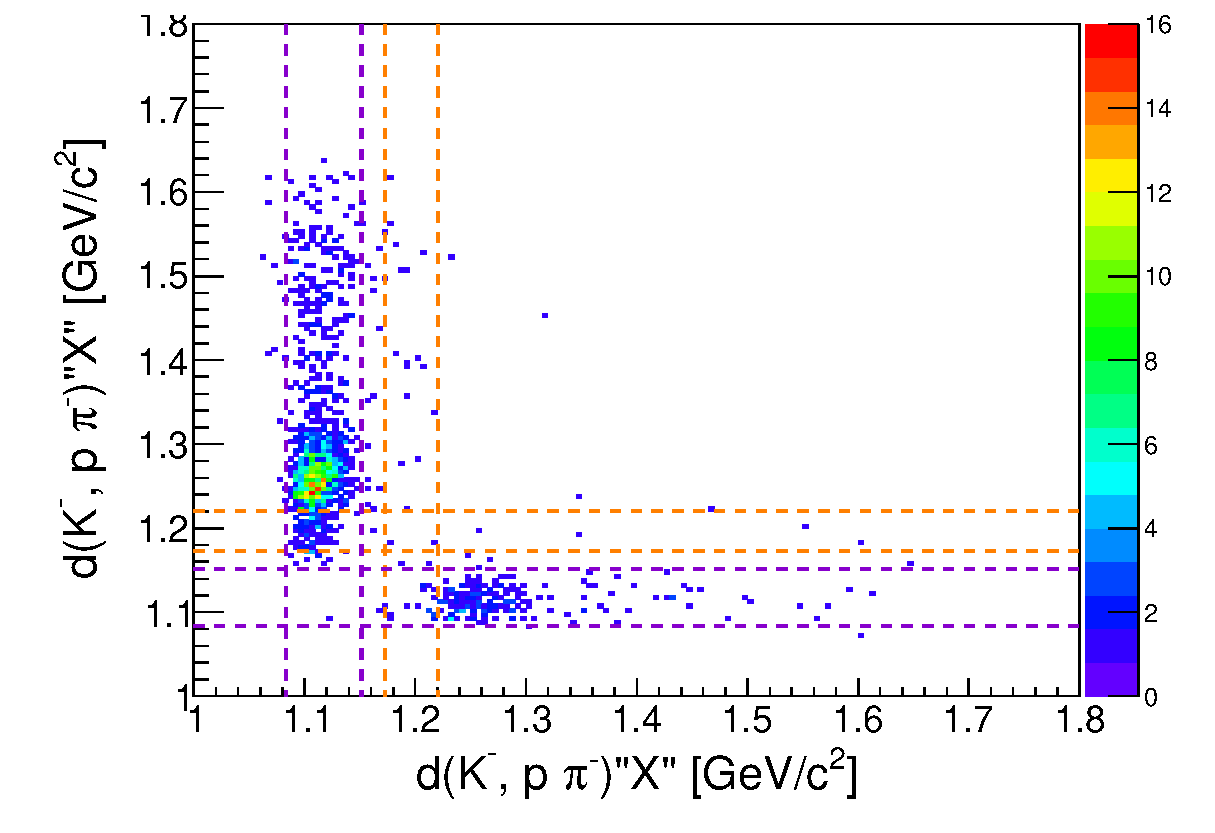
\includegraphics[width=5cm]{../pic/Run68/KP_ana/KPpim_KPpim_MM_mmP.eps}
    \end{minipage}
    \begin{minipage}{0.5\hsize}
      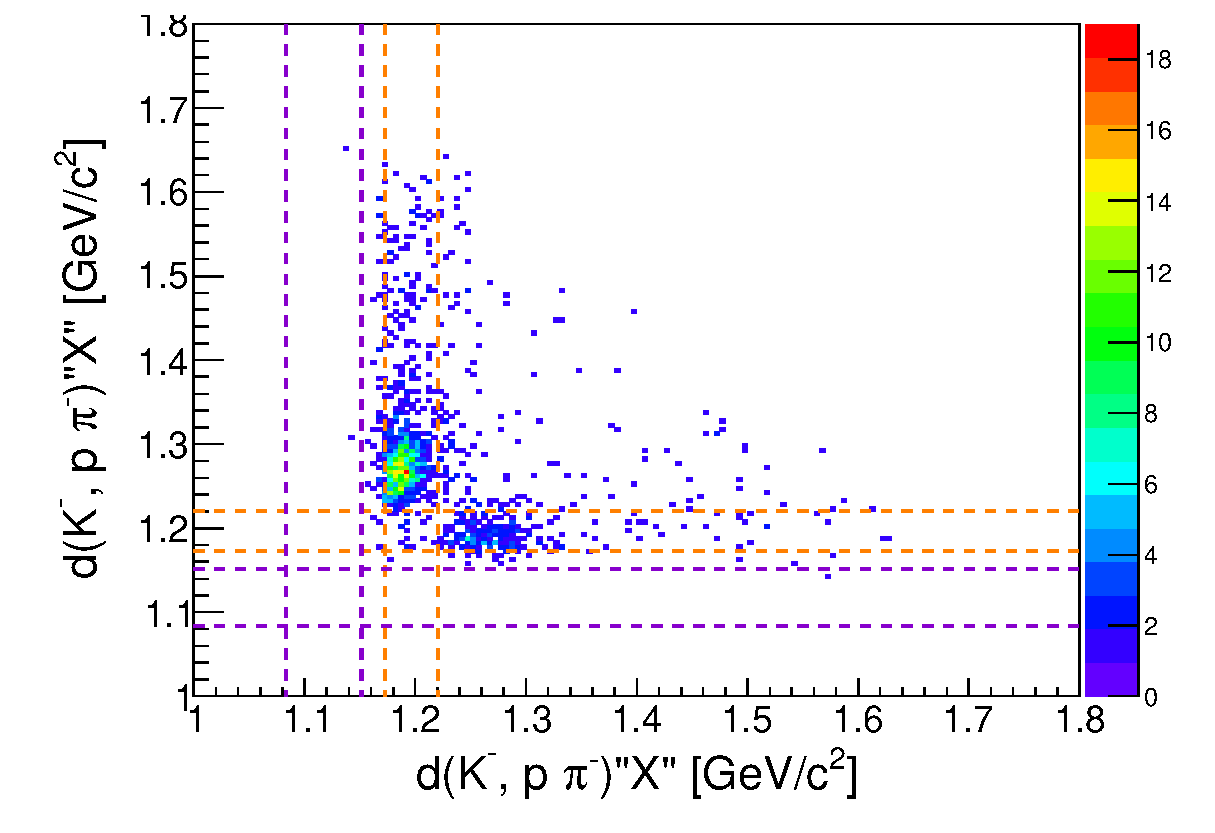
\includegraphics[width=5cm]{../pic/Run68/KP_ana/KPpim_KPpim_MM_mmPgamma.eps}
    \end{minipage}
  \end{tabular}
  \caption{
    These figures shows same figure of Fig\ref{fig:KPpim_KPpim} excepting $d(K^-, p \pi^- \pi^-)$ tag.
    Left figure shows $d(K^-, p \pi^- \pi^-)"p"$ tagged events and right figure shows $d(K^-, p \pi^- \pi^-)"p \gamma"$ tagged events.
  }
  \label{fig:KPpim_KPpim_wTag}
\end{figure}

\begin{figure}[htbp]
  \centering
  \begin{tabular}{cc}
    \begin{minipage}{0.5\hsize}
      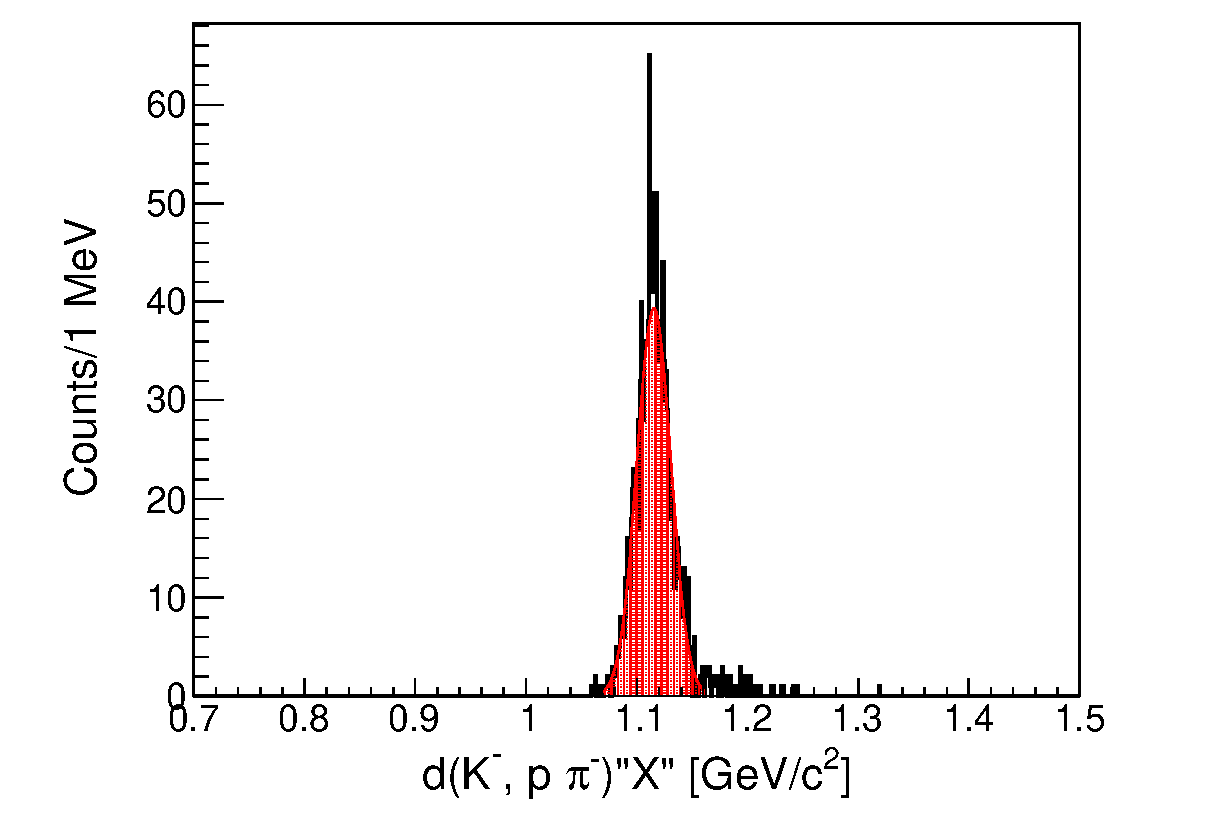
\includegraphics[width=5cm]{../pic/Run68/KP_ana/KPpim_MM_Lmass.eps}
    \end{minipage}
    \begin{minipage}{0.5\hsize}
      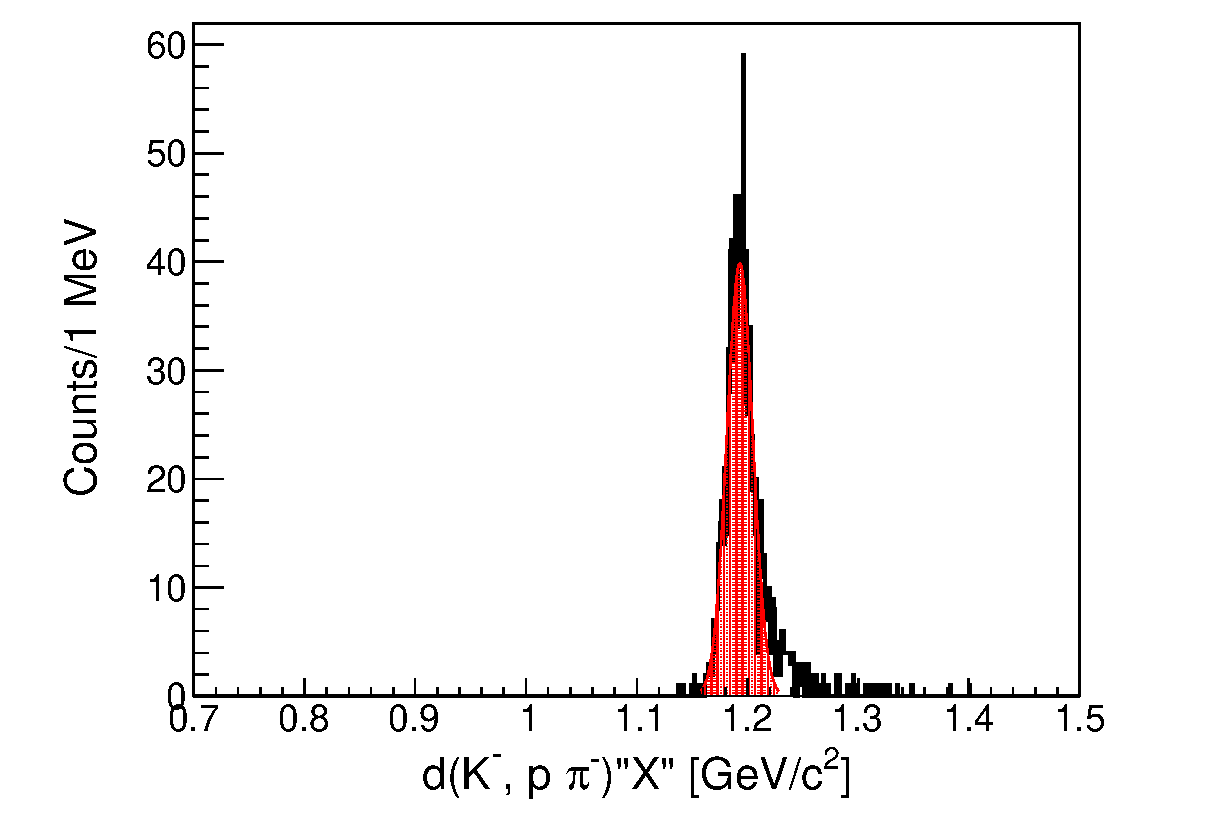
\includegraphics[width=5cm]{../pic/Run68/KP_ana/KPpim_MM_S0mass.eps}
    \end{minipage}
  \end{tabular}
  \caption{
    This figure indicate 1 dimensional plots of Fig\ref{fig:KPpim_KPpim_wTag}.
    Only near pair from PDG mass was filled histogram.
    These mass is $\Lambda$ and $\Sigma^{0}$ left and right respectively.
  }
  \label{fig:KPpim_wTag}
\end{figure}

The $d(K^-, p)"\pi-\Sigma^0"$ and the $d(K^-, p)"\pi^-\Lambda"$ final states were indetified from the following decay chains.

\begin{eqnarray}
  K^- d \rightarrow p \pi^- \Sigma^0 \rightarrow p \pi^- \gamma \Lambda \rightarrow p \pi^- \pi^- \gamma p \label{eq:KP_pimS0}\\
  K^- d \rightarrow p \pi^- \Lambda \rightarrow p \pi^- \pi^- p \label{eq:KP_pimL}
\end{eqnarray}

These final states were searched from the events detecting the proton by forward detectors and 2$\pi^-$- by the CDS which adopted the offline analysis selection for the rejection of the accidental.
The final states were identified from both hyperon identification and proton identification.
% To do add appendix 
In the $d(K^-, p)"\pi^- \Lambda"$ mode, the missing proton was identified from the $d(K^-, p \pi^- \pi^-)$ .
On the other hand, in the $d(K^-, p)"\Sigma^0"$ mode, that was the proton and $\gamma$ events, which were shown in Fig\ref{fig:KPpimpim}.
Two types of the $d(K^-, p \pi^-)$ missing masses can be combined due to two $\pi^-$, which was shown in Fig\ref{fig:KPpim_KPpim_wTag}.
In these figures, the orange lines indicate $d(K^-, p \pi^-)"\pi^-\Sigma^0"$ selections and the purple lines indicate $d(K^-, p \pi^-)"\pi^-\Lambda"$ selections.
The same plots with the $d(K^-, p \pi^- \pi^-)"p"$ selection and the $d(K^-, p \pi^- \pi^-)"p \gamma"$ selection were shown in the left figure and the right figure of Fig\ref{fig:KPpim_wTag},
respectively.

The $d(K^-, p \pi^- \pi^-)"p"$ peak, the $d(K^-, p \pi^-)"\Sigma^0"$ peak, and the $d(K^-, p \pi^-)"\Lambda"$ peak were used for the time offset calibration
which was described at Sec\ref{sec:KP_timeoffset}.
Fig\ref{fig:KPpim_wTag} shows the $d(K^-, p \pi^-)"\Sigma^0"$ peak and the $d(K^-, p \pi^-)"\Lambda"$ missing mass peaks in the left figure and the right figure, respectively.
These were made to select near the PDG value in each event.\\
Obtained the $d(K^-, p)"\pi^- \Sigma^0$ and the $d(K^-, p)"\pi^- \Lambda"$ spectra were shown in Fig\ref{fig:KP_MM_piY}.
% which were corrected by the acceptance estimated by the MC sim and convert to cross section using luminosity and the detector efficiency.

\begin{figure}[htbp]
  \begin{tabular}{cc}
    \begin{minipage}{0.5\hsize}
      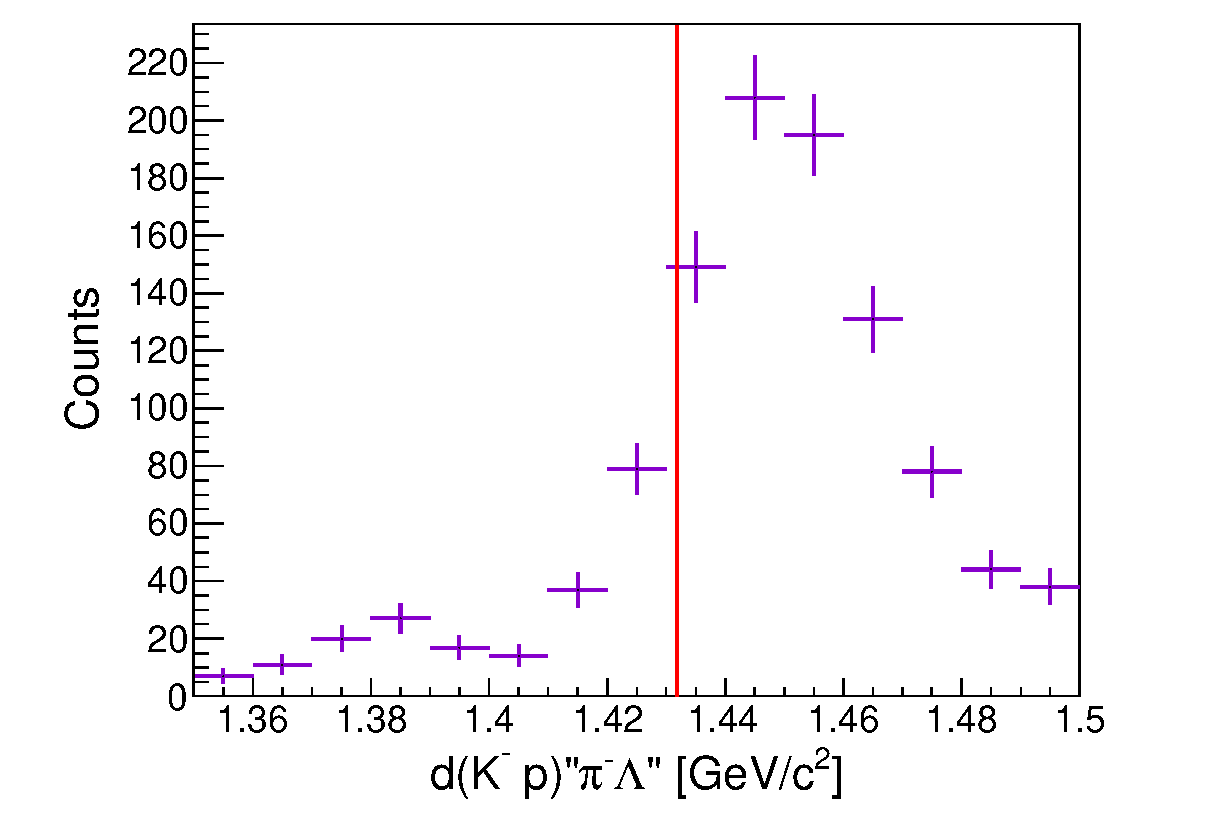
\includegraphics[width=7cm]{../pic/Dron/KP_ana/KP_MM_pimL.eps}
    \end{minipage}

    \begin{minipage}{0.5\hsize}
      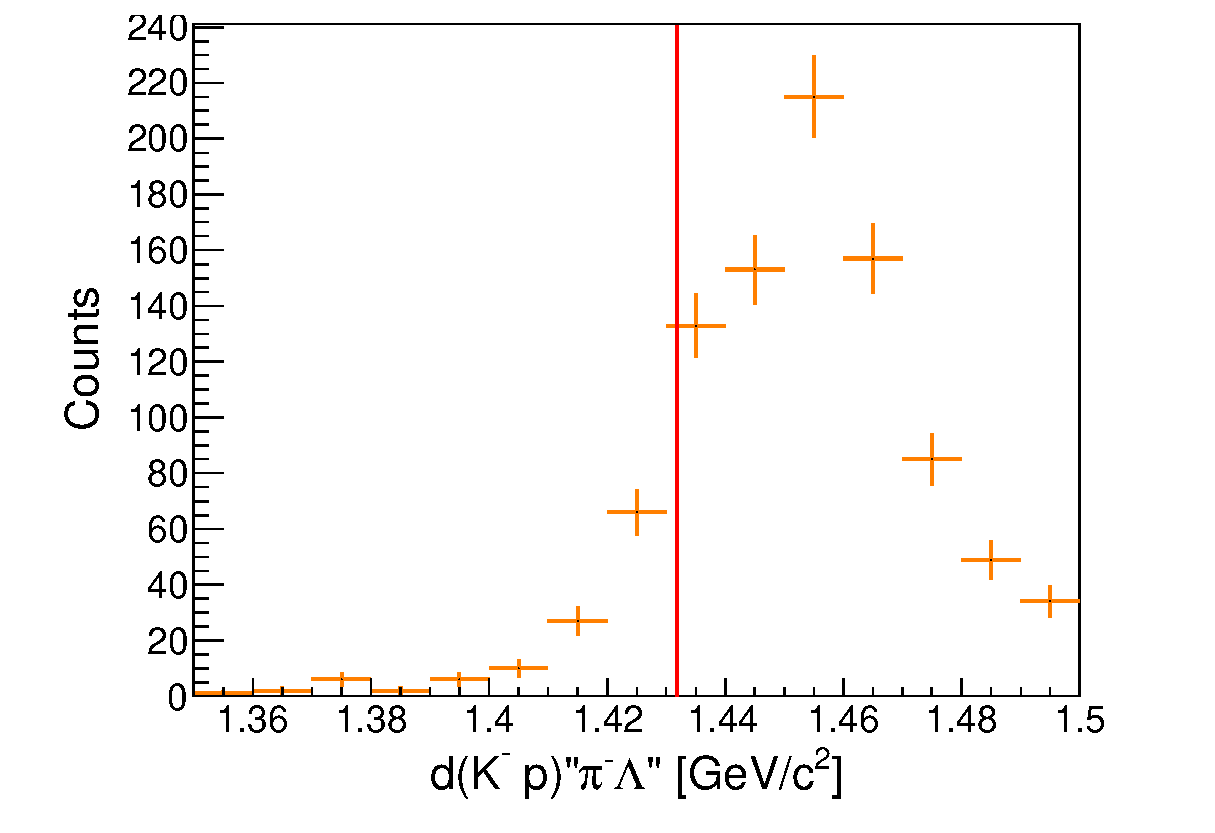
\includegraphics[width=7cm]{../pic/Dron/KP_ana/KP_MM_pimS0.eps}
    \end{minipage}
  \end{tabular}
  \caption{
    Left figure shows $d(K^-, p)"\pi^-\Lambda"$ and Right figure shows $d(K^-, p)"\pi^-\Sigma^0"$
  }
  \label{fig:KP_MM_piY}
\end{figure}
